\chapter{Technologieën}
\label{ch:technologies}
Alle technologieën hieronder besproken zijn allemaal vrij simpel vervangbaar in een modulair systeem zoals LangChain.

\section{Backend}
\subsection{Databases}
Een van de belangrijkste componenten van een chatbot die gebouwd is voor specifieke doeleinden, is een plaats om data te kunnen opslaan.
Een gesprek met een RAG app kan schematisch voorgesteld worden als volgt:

\begin{figure}[h]
	\makebox[\textwidth] {
		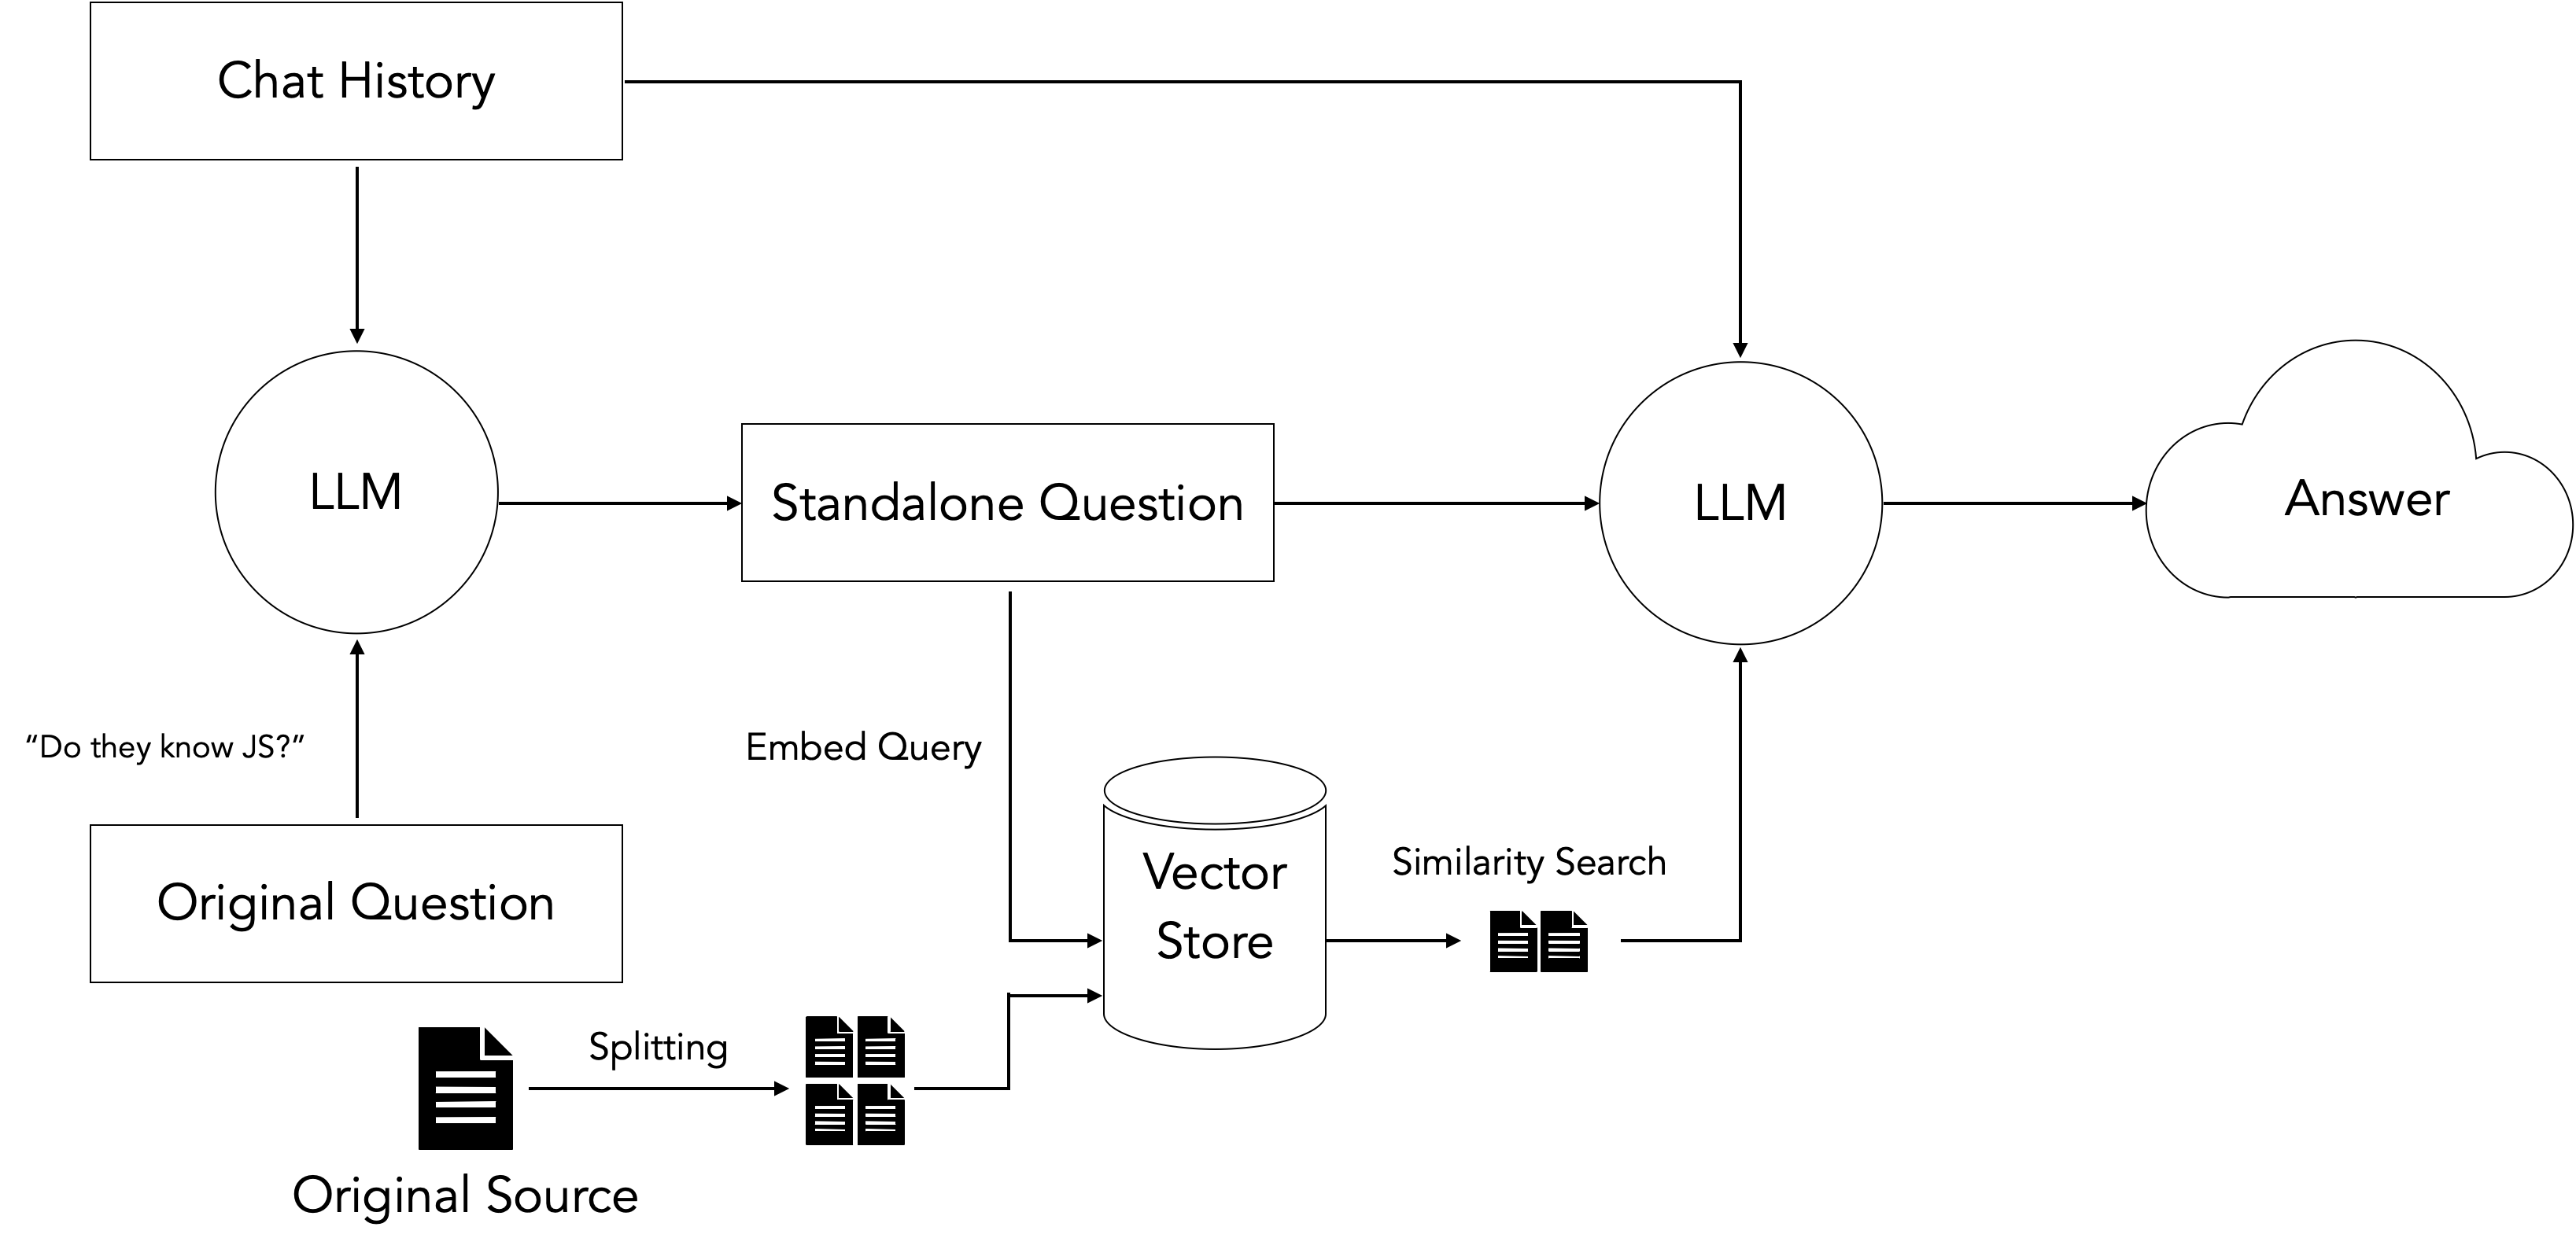
\includegraphics[width=\textwidth]{llm_pipeline.png}
	}
	\captionof{figure}{Schematische voorstelling van een conversatie met een LLM chatbot \autocite{Ollama} }
\end{figure}

Hier valt op dat een LLM niet alleen de vraag van de gebruiker in acht neemt, maar ook relevante documenten opvraagt uit een Vector store. 

\subsubsection{Vectorstore: Chroma}
De eerste keuze die moet worden gemaakt is welke vectorstore te gebruiken. Veel bronnen op het web bespreken open-source databases zoals Weaviate, Opensearch, Qdrant en Chroma. 
Chroma biedt ondersteuning met LangChain en kan gemakkelijk lokaal gedraaid worden. 
Chroma is de keuze die door LangChain aangeraden wordt als lokaal alternatief voor een online instantie van Weaviate.  
Omdat we met gevoelige documenten werken, willen we Deltalex Chat graag volledig lokaal houden dus vandaar zullen we voor Chroma kiezen als onze lokale vectorstore. 

\subsubsection{Record store: Postgres}
Een vectorstore is een grote ongestructureerde ruimte met alle berekende vectoren en documentdata. 
Het kan handig zijn om naast deze ruimte een externe database bij te houden die bijvoorbeeld transactionele data (welke documenten er in de vectorstore zijn gegaan en wanneer), 
gebruikersdata en andere gestructureerde data bijhoudt. Dit is in ons proof-of-concept niet van gigantisch belang dus houden we het hier op een simpele open-source database genaamd Postgres. 

\subsection{Centraal verwerkingssysteem}
Om alles samen te gieten en te beheren, hebben we een modulair systeem nodig dat we ofwel volledig zelf kunnen bouwen, of kunnen overnemen van een open-source framework. 
Eén van de populairste én best gedocumenteerde frameworks hiervoor is LangChain. 
De missie van Langchain is om de volledige levenscyclus van AI systemen makkelijker te maken om te beheren. 
Zo kan men zijn eigen systeem schrijven met modulaire bouwblokken die allemaal open-source zijn en dit integreren met third-party clients zoals AWS, Google, OpenAI, ... \\ 

De keuze voor Deltalex Chat zal dan ook naar LangChain gaan omdat het heel flexibel is. 
Allerbelangrijkst is het ook volledig lokaal draaibaar en open-source. 

\newpage
\subsection{Modelkeuze en beheer}
Een van de belangrijkste componenten van een digitale assistent is vanzelfsprekend artificiële intelligentie. 
Er wordt op twee plaatsen in de toepassing gebruikt gemaakt van AI: 

\begin{itemize}
	\item Tijdens het genereren van embeddings
	\item Tijdens het chatten en genereren van documenten
\end{itemize}

Voor deze twee doelen hebben we twee verschillende modellen nodig. 
Omdat alles lokaal zal draaien, hebben we een toepassing nodig op ons systeem om modellen te draaien en te beheren. 
Een toepassing die de laatste tijd heel erg populair aan het worden is in de open-source AI wereld, is Ollama. 
Ollama is een programma dat toestaat als gebruiker (via command line) modellen lokaal te downloaden, beheren en te draaien. 
De modellen kunnen via een interactieve Python prompt gebruikt worden of via een exposed API. 
Dit maakt het mogelijk om (via een community plugin) aangesproken te worden door LangChain. 

\subsubsection{Embedding model}
Het is niet mogelijk om documenten rechtstreeks in een vectorstore te plaatsen. 
Er moeten eerst van die documenten vectoren berekend worden waarop de vectorstore kan berekenen of een stuk tekst relevant is met de query van de gebruiker of niet. 
Om deze te berekenen, wordt er gebruik gemaakt van een text-embedding model. Dit zal de tekstuele informatie overzetten naar dergelijke vectoren die compatibel zijn met Chroma. 

Er zijn veel embedding modellen beschikbaar via Ollama, waarvan het populairste \textbf{nomic-embed-text}. 
Nomic heeft tot nu toe al rond de 350 duizend downloads van Ollama en is dus veruit het meest gedownloade. 
De keuze hiervoor is dan ook snel gemaakt. 

\subsubsection{large language model}
Large Language Models zijn de laatste tijd gigantisch populair geworden door bv. ChatGPT van OpenAI.
Hun bijna menselijke interactie zorgt ervoor dat een gebruiker de indruk heeft dat hij aan het praten is met een menselijke assistent maar dan veel sneller en 'slimmer'.

Natuurlijk is niets minder waar.
Een Large Language Model is immers een soort transformer, die de input (of query) van een gebruiker 'transformeert' naar een antwoord door de volgende token (woord) te voorspellen.
Deze modellen kunnen gegeneraliseerd worden voor verschillende use cases, niet zoals hun voorgangers zoals een PLM (Pretrained Language Model).
Het verschil hier is vooral de gigantische dataset waarop LLM's getrained worden.
Dit maakt ze toepasbaar op een veel breder gebied zonder enige extra configuratie of aanpassing.

Er zijn de laatste tijd heel veel modellen (zowel open- als closed-source) op de markt gekomen. Dit maakt het moeilijk om te kiezen voor een large-language-model voor onze implementatie. 
Volgens populariteit bij het ollama modelregister zijn llama3, Gemma, Qwen en Mistral de bekendste. De eerste drie zijn van Meta, Google en Alibaba. \\

In deze proof-of-concept zal Mistral gebruikt worden. Het is natuurlijk altijd mogelijk om te testen tussen verschillende modellen om te zien wat de advocaat in kwestie verkiest. 

\section{Frontend}
Het is natuurlijk niet echt aantrekkelijk voor een advocaat om alles te doen via command line aangezien dit voor hun niet echt intuïtief en gebruiksvriendelijk is. 
Daarom is het maken van een aantrekkelijke en gebruiksvriendelijke frontend een absolute must in onze POC. \\ 

Er zijn heel veel repositories online die al een vooraf geïmplementeerde chat-interface die makkelijk via een NodeJS library kan gerund en getest worden. 
Deze oplossingen bieden een goede basis voor de ontwikkeling van een frontend, maar moeten aangepast en aangepast worden om te conformeren aan de huisstijl van Deltalex en zodat ze alleen maar het absolute nodige weergeven. \\

In het volgende hoofdstuk zullen we verder ingaan op de implementatie van de frontend. 
We zullen met screenshots de werking verduidelijken en uitleggen. 
